%%**************************************************************
%% Vorlage fuer Bachelorarbeiten (o.ä.) der DHBW
%%
%% Autor: Tobias Dreher, Yves Fischer
%% Datum: 06.07.2011
%%
%% Autor: Michael Gruben
%% Datum: 15.05.2013
%%
%% Autor: Markus Barthel
%% Datum: 22.08.2014
%%**************************************************************

%!TEX root = ../dokumentation.tex

%
% Nahezu alle Einstellungen koennen hier getaetigt werden
%

\RequirePackage[l2tabu, orthodox]{nag}	% weist in Commandozeile bzw. log auf veraltete LaTeX Syntax hin

\documentclass[%
	pdftex,
	oneside,			% Einseitiger Druck.
	13pt,				% Schriftgroesse
	parskip=half,		% Halbe Zeile Abstand zwischen Absätzen.
%	topmargin = 10pt,	% Abstand Seitenrand (Std:1in) zu Kopfzeile [laut log: unused]
	headheight = 12pt,	% Höhe der Kopfzeile
%	headsep = 30pt,	% Abstand zwischen Kopfzeile und Text Body  [laut log: unused]
	headsepline,		% Linie nach Kopfzeile.
	footsepline,		% Linie vor Fusszeile.
	footheight = 16pt,	% Höhe der Fusszeile
	abstracton,		% Abstract Überschriften
	DIV=calc,		% Satzspiegel berechnen
	BCOR=8mm,		% Bindekorrektur links: 8mm
	headinclude=false,	% Kopfzeile nicht in den Satzspiegel einbeziehen
	footinclude=false,	% Fußzeile nicht in den Satzspiegel einbeziehen
	listof=totoc,		% Abbildungs-/ Tabellenverzeichnis im Inhaltsverzeichnis darstellen
	toc=bibliography,	% Literaturverzeichnis im Inhaltsverzeichnis darstellen
]{scrreprt}	% Koma-Script report-Klasse, fuer laengere Bachelorarbeiten alternativ auch: scrbook

% Einstellungen laden
\usepackage{xstring}
\usepackage[utf8]{inputenc}
\usepackage[T1]{fontenc}

\newcommand{\einstellung}[1]{%
  \expandafter\newcommand\csname #1\endcsname{}
  \expandafter\newcommand\csname setze#1\endcsname[1]{\expandafter\renewcommand\csname#1\endcsname{##1}}
}
\newcommand{\langstr}[1]{\einstellung{lang#1}}

\einstellung{martrikelnr}
\einstellung{titel}
\einstellung{kurs}
\einstellung{datumAbgabe}
\einstellung{firma}
\einstellung{firmenort}
\einstellung{abgabeort}
\einstellung{abschluss}
\einstellung{studiengang}
\einstellung{dhbw}
\einstellung{betreuer}
\einstellung{gutachter}
\einstellung{zeitraum}
\einstellung{arbeit}
\einstellung{autor}
\einstellung{sprache}
\einstellung{schriftart}
\einstellung{seitenrand}
\einstellung{kapitelabstand}
\einstellung{spaltenabstand}
\einstellung{zeilenabstand}
\einstellung{zitierstil}
 % verfügbare Einstellungen
%%%%%%%%%%%%%%%%%%%%%%%%%%%%%%%%%%%%%%%%%%%%%%%%%%%%%%%%%%%%%%%%%%%%%%%%%%%%%%%
%                                   Einstellungen
%
% Hier können alle relevanten Einstellungen für diese Arbeit gesetzt werden.
% Dazu gehören Angaben u.a. über den Autor sowie Formatierungen.
%
%
%%%%%%%%%%%%%%%%%%%%%%%%%%%%%%%%%%%%%%%%%%%%%%%%%%%%%%%%%%%%%%%%%%%%%%%%%%%%%%%


%%%%%%%%%%%%%%%%%%%%%%%%%%%%%%%%%%%% Sprache %%%%%%%%%%%%%%%%%%%%%%%%%%%%%%%%%%%
%% Aktuell sind Deutsch und Englisch unterstützt.
%% Es werden nicht nur alle vom Dokument erzeugten Texte in
%% der entsprechenden Sprache angezeigt, sondern auch weitere
%% Aspekte angepasst, wie z.B. die Anführungszeichen und
%% Datumsformate.
\setzesprache{de} % oder en
%%%%%%%%%%%%%%%%%%%%%%%%%%%%%%%%%%%%%%%%%%%%%%%%%%%%%%%%%%%%%%%%%%%%%%%%%%%%%%%%

%%%%%%%%%%%%%%%%%%%%%%%%%%%%%%%%%%% Angaben  %%%%%%%%%%%%%%%%%%%%%%%%%%%%%%%%%%%
%% Die meisten der folgenden Daten werden auf dem
%% Deckblatt angezeigt, einige auch im weiteren Verlauf
%% des Dokuments.
\setzemartrikelnr{5946066,XXXXX}
\setzekurs{STG-TINF17-ITA}
\setzetitel{Chat und 4-gewinnt-Spiel mit Docker und Node.js}
\setzedatumAbgabe{12.06.2019}
\setzefirma{Daimler AG}
\setzefirmenort{Stuttgart}
\setzeabgabeort{Stuttgart}
\setzeabschluss{nothing}
\setzestudiengang{Informatik/IT-Automotive}
\setzedhbw{Stuttgart}
\setzebetreuer{nothing}
\setzegutachter{nothing}
\setzezeitraum{nothing}
\setzearbeit{Projekdokumentation Microservices}
\setzeautor{Hanna Siegfried und Nahku Saidy}
%%%%%%%%%%%%%%%%%%%%%%%%%%%%%%%%%%%%%%%%%%%%%%%%%%%%%%%%%%%%%%%%%%%%%%%%%%%%%%%%

%%%%%%%%%%%%%%%%%%%%%%%%%%%% Literaturverzeichnis %%%%%%%%%%%%%%%%%%%%%%%%%%%%%%
%% Bei Fehlern während der Verarbeitung bitte in ads/header.tex bei der
%% Einbindung des Pakets biblatex (ungefähr ab Zeile 110,
%% einmal für jede Sprache), biber in bibtex ändern.
\newcommand{\ladeliteratur}{%
\addbibresource{bibliographie.bib}
%\addbibresource{weitereDatei.bib}
}

%% Zitierstil
%% siehe: http://ctan.mirrorcatalogs.com/macros/latex/contrib/biblatex/doc/biblatex.pdf (3.3.1 Citation Styles)
%% mögliche Werte z.B numeric-comp, alphabetic, authoryear
\setzezitierstil{numeric}
%%%%%%%%%%%%%%%%%%%%%%%%%%%%%%%%%%%%%%%%%%%%%%%%%%%%%%%%%%%%%%%%%%%%%%%%%%%%%%%%

%%%%%%%%%%%%%%%%%%%%%%%%%%%%%%%%% Layout %%%%%%%%%%%%%%%%%%%%%%%%%%%%%%%%%%%%%%%
%% Verschiedene Schriftarten
% laut nag Warnung: palatino obsolete, use mathpazo, helvet (option scaled=.95), courier instead
\setzeschriftart{lmodern} % palatino oder goudysans, lmodern, libertine

%% Paket um Textteile drehen zu können
%\usepackage{rotating}
%% Paket um Seite im Querformat anzuzeigen
%\usepackage{lscape}

%% Seitenränder
\setzeseitenrand{2.5cm}

%% Abstand vor Kapitelüberschriften zum oberen Seitenrand
\setzekapitelabstand{20pt}

%% Spaltenabstand
\setzespaltenabstand{10pt}
%%Zeilenabstand innerhalb einer Tabelle
\setzezeilenabstand{1.5}
%%%%%%%%%%%%%%%%%%%%%%%%%%%%%%%%%%%%%%%%%%%%%%%%%%%%%%%%%%%%%%%%%%%%%%%%%%%%%%%%

%%%%%%%%%%%%%%%%%%%%%%%%%%%%% Verschiedenes  %%%%%%%%%%%%%%%%%%%%%%%%%%%%%%%%%%%
%% Farben (Angabe in HTML-Notation mit großen Buchstaben)
\newcommand{\ladefarben}{%
	\definecolor{LinkColor}{HTML}{00007A}
	\definecolor{ListingBackground}{HTML}{FCFAFB}
}
%% Mathematikpakete benutzen (Pakete aktivieren)
\usepackage{amsmath}
\usepackage{amssymb}

%% Programmiersprachen Highlighting (Listings)
\newcommand{\listingsettings}{%
	\lstset{%
		language=Java,			% Standardsprache des Quellcodes
		numbers=left,			% Zeilennummern links
		stepnumber=1,			% Jede Zeile nummerieren.
		numbersep=5pt,			% 5pt Abstand zum Quellcode
		numberstyle=\tiny,		% Zeichengrösse 'tiny' für die Nummern.
		breaklines=true,		% Zeilen umbrechen wenn notwendig.
		breakautoindent=true,	% Nach dem Zeilenumbruch Zeile einrücken.
		postbreak=\space,		% Bei Leerzeichen umbrechen.
		tabsize=2,				% Tabulatorgrösse 2
		basicstyle=\ttfamily\footnotesize, % Nichtproportionale Schrift, klein für den Quellcode
		showspaces=false,		% Leerzeichen nicht anzeigen.
		showstringspaces=false,	% Leerzeichen auch in Strings ('') nicht anzeigen.
		extendedchars=true,		% Alle Zeichen vom Latin1 Zeichensatz anzeigen.
		captionpos=b,			% sets the caption-position to bottom
		backgroundcolor=\color{ListingBackground}, % Hintergrundfarbe des Quellcodes setzen.
		xleftmargin=0pt,		% Rand links
		xrightmargin=0pt,		% Rand rechts
		frame=single,			% Rahmen an
		frameround=ffff,
		rulecolor=\color{darkgray},	% Rahmenfarbe
		fillcolor=\color{ListingBackground},
		keywordstyle=\color[rgb]{0.133,0.133,0.6}\bfseries,
		commentstyle=\color{Sepia},
		stringstyle=\color{red}
	}
}
%%%%%%%%%%%%%%%%%%%%%%%%%%%%%%%%%%%%%%%%%%%%%%%%%%%%%%%%%%%%%%%%%%%%%%%%%%%%%%%%

%%%%%%%%%%%%%%%%%%%%%%%%%%%%%%%% Eigenes %%%%%%%%%%%%%%%%%%%%%%%%%%%%%%%%%%%%%%%
%% Hier können Ergänzungen zur Präambel vorgenommen werden (eigene Pakete, Einstellungen)

% xcolor muss mit optionen vor pdfpages geladen werden
\usepackage[usenames,dvipsnames,table,xcdraw]{xcolor} 	%xcolor für HTML-Notation

\usepackage{pdfpages}
 % lese Einstellungen

\newcommand{\iflang}[2]{%
  \IfStrEq{\sprache}{#1}{#2}{}
}

\langstr{abkverz}
\langstr{anhang}
\langstr{glossar}
\langstr{deckblattabschlusshinleitung}
\langstr{artikelstudiengang}
\langstr{studiengang}
\langstr{anderdh}
\langstr{von}
\langstr{dbbearbeitungszeit}
\langstr{dbmatriknr}
\langstr{dbkurs}
\langstr{dbfirma}
\langstr{dbbetreuer}
\langstr{dbgutachter}
\langstr{sperrvermerk}
\langstr{erklaerung}
\langstr{abstract}
\langstr{listingname}
\langstr{listlistingname}
\langstr{listingautorefname}
 % verfügbare Strings
\input{lang/\sprache} % Übersetzung einlesen

% Einstellung der Sprache des Paketes Babel und der Verzeichnisüberschriften
\iflang{de}{\usepackage[english, ngerman]{babel}}
\iflang{en}{\usepackage[ngerman, english]{babel}} 


%%%%%%% Package Includes %%%%%%%

\usepackage[margin=\seitenrand,foot=1cm]{geometry}	% Seitenränder und Abstände
\usepackage[activate]{microtype} %Zeilenumbruch und mehr
\usepackage[onehalfspacing]{setspace}
\usepackage{makeidx}
\usepackage[autostyle=true,german=quotes]{csquotes}
\usepackage{tabularx}
\usepackage{longtable}
\usepackage{multirow}
\usepackage{enumitem}	% mehr Optionen bei Aufzählungen
\usepackage{graphicx}
%\usepackage[usenames,dvipsnames,table,xcdraw]{xcolor} 	%xcolor für HTML-Notation
\usepackage{float}
\usepackage{array}
\usepackage{calc}		% zum Rechnen (Bildtabelle in Deckblatt)
\usepackage[right]{eurosym}
\usepackage{wrapfig}
\usepackage{pgffor} % für automatische Kapiteldateieinbindung
\usepackage[perpage, hang, multiple, stable]{footmisc} % Fussnoten
%\usepackage[nohyperlinks]{acronym} % falls gewünscht kann die Option footnote eingefügt werden, dann wird die Erklärung nicht inline sondern in einer Fußnote dargestellt
%\usepackage[printonlyused,footnote]{acronym}
\usepackage{acronym}


%\usepackage{algorithm}
\usepackage[Algorithmus]{algorithm}
\usepackage{algorithmic}

\renewcommand{\algorithmicrequire}{\textbf{Eingabe:}} 
\renewcommand{\algorithmicensure}{\textbf{Ausgabe:}} 


\usepackage{listings}

% Eigene zusätzliche packages
\usepackage{xfrac}
\usepackage{tikz}
\usepackage{subcaption}
%\usepackage[leqno]{amsmath}
%\usepackage{remreset}

% Wurzel mit schießendem Strich am ende
% New definition of square root: % it renames \sqrt as \oldsqrt
\let\oldsqrt\sqrt % it defines the new \sqrt in terms of the old one 
\def\sqrt{\mathpalette\DHLhksqrt} \def\DHLhksqrt#1#2{
\setbox0=\hbox{$#1\oldsqrt{#2\,}$}\dimen0=\ht0 \advance\dimen0-0.2\ht0 \setbox2=\hbox{\vrule height\ht0 depth -\dimen0}{\box0\lower0.4pt\box2}}

%\makeatletter
%\@removefromreset{equation}{chapter}
%\makeatother
%\renewcommand*{\theequation}{\arabic{equation}}

% eine Kommentarumgebung "k" (Handhabe mit \begin{k}<Kommentartext>\end{k},
% Kommentare werden rot gedruckt). Wird \% vor excludecomment{k} entfernt,
% werden keine Kommentare mehr gedruckt.
\usepackage{comment}
\specialcomment{k}{\begingroup\color{red}}{\endgroup}
%\excludecomment{k}


%%%%%% Configuration %%%%%

%% Anwenden der Einstellungen

\usepackage{\schriftart}
\ladefarben{}

% Titel, Autor und Datum
\title{\titel}
\author{\autor}
\date{\datum}

% PDF Einstellungen
\usepackage[%
	pdftitle={\titel},
	pdfauthor={\autor},
	pdfsubject={\arbeit},
	pdfcreator={pdflatex, LaTeX with KOMA-Script},
	pdfpagemode=UseOutlines, 		% Beim Oeffnen Inhaltsverzeichnis anzeigen
	pdfdisplaydoctitle=true, 		% Dokumenttitel statt Dateiname anzeigen.
	pdflang={\sprache}, 			% Sprache des Dokuments.
]{hyperref}

% (Farb-)einstellungen für die Links im PDF
\hypersetup{%
	colorlinks=true, 		% Aktivieren von farbigen Links im Dokument
	linkcolor=LinkColor, 	% Farbe festlegen
	citecolor=LinkColor,
	filecolor=LinkColor,
	menucolor=LinkColor,
	urlcolor=LinkColor,
	linktocpage=true, 		% Nicht der Text sondern die Seitenzahlen in Verzeichnissen klickbar
	bookmarksnumbered=true 	% Überschriftsnummerierung im PDF Inhalt anzeigen.
}
% Workaround um Fehler in Hyperref, muss hier stehen bleiben
\usepackage{bookmark} %nur ein latex-Durchlauf für die Aktualisierung von Verzeichnissen nötig

% Schriftart in Captions etwas kleiner
\addtokomafont{caption}{\small}

% Literaturverweise (sowohl deutsch als auch englisch)
\iflang{de}{%
\usepackage[
	backend=biber,		% empfohlen. Falls biber Probleme macht: bibtex
	bibwarn=true,
	sorting=none,
	bibencoding=utf8,	% wenn .bib in utf8, sonst ascii
	sortlocale=de_DE,
	maxbibnames=99,
	style=\zitierstil,
	backref=false %keine Rückverweise
]{biblatex}
}
\iflang{en}{%
\usepackage[
	backend=biber,		% empfohlen. Falls biber Probleme macht: bibtex
	bibwarn=true,
	sorting=none,
	bibencoding=utf8,	% wenn .bib in utf8, sonst ascii
	sortlocale=en_US,
	maxbibnames=99,
	style=\zitierstil,
	backref=false %keine Rückverweise
]{biblatex}
}

% Mehr Platz zwischen einzelnen Items im Literaturverzeichnis bei Verwendung von authoryear
\setlength{\bibitemsep}{\baselineskip}
\DeclareNameAlias{sortname}{last-first}

\ladeliteratur{}

% Glossar
\usepackage[nonumberlist,toc,section=chapter,nomain,nopostdot]{glossaries}

%%%%%% Additional settings %%%%%%

% Hurenkinder und Schusterjungen verhindern
% http://projekte.dante.de/DanteFAQ/Silbentrennung
\clubpenalty = 10000 % schließt Schusterjungen aus (Seitenumbruch nach der ersten Zeile eines neuen Absatzes)
\widowpenalty = 10000 % schließt Hurenkinder aus (die letzte Zeile eines Absatzes steht auf einer neuen Seite)
\displaywidowpenalty=10000

% Bildpfad
\graphicspath{{images/}}

% Einige häufig verwendete Sprachen
\lstloadlanguages{PHP,Python,Java,C,C++,bash,XML}
\listingsettings{}
% Umbennung des Listings
\renewcommand\lstlistingname{\langlistingname}
\renewcommand\lstlistlistingname{\langlistlistingname}
\def\lstlistingautorefname{\langlistingautorefname}

% Umlaute ermöglichen in listings
\lstset{literate=
	{á}{{\'a}}1 {é}{{\'e}}1 {í}{{\'i}}1 {ó}{{\'o}}1 {ú}{{\'u}}1
	{Á}{{\'A}}1 {É}{{\'E}}1 {Í}{{\'I}}1 {Ó}{{\'O}}1 {Ú}{{\'U}}1
	{à}{{\`a}}1 {è}{{\`e}}1 {ì}{{\`i}}1 {ò}{{\`o}}1 {ù}{{\`u}}1
	{À}{{\`A}}1 {È}{{\'E}}1 {Ì}{{\`I}}1 {Ò}{{\`O}}1 {Ù}{{\`U}}1
	{ä}{{\"a}}1 {ë}{{\"e}}1 {ï}{{\"i}}1 {ö}{{\"o}}1 {ü}{{\"u}}1
	{Ä}{{\"A}}1 {Ë}{{\"E}}1 {Ï}{{\"I}}1 {Ö}{{\"O}}1 {Ü}{{\"U}}1
	{â}{{\^a}}1 {ê}{{\^e}}1 {î}{{\^i}}1 {ô}{{\^o}}1 {û}{{\^u}}1
	{Â}{{\^A}}1 {Ê}{{\^E}}1 {Î}{{\^I}}1 {Ô}{{\^O}}1 {Û}{{\^U}}1
	{œ}{{\oe}}1 {Œ}{{\OE}}1 {æ}{{\ae}}1 {Æ}{{\AE}}1 {ß}{{\ss}}1
	{ç}{{\c c}}1 {Ç}{{\c C}}1 {ø}{{\o}}1 {å}{{\r a}}1 {Å}{{\r A}}1
	{€}{{\EUR}}1 {£}{{\pounds}}1
}

% Weitere Keyword Highlights
\lstset{
	emph=[1]{ 
	    mkdir, jps, sudo, wget, mv, chown, su, adduser, addgroup, grep, sort, print, max, WARNING
    },
    emphstyle=[1]{\color[rgb]{0.133,0.133,0.6}},
    emph=[2]{
	    LFAConfiguration, Driver, Set, Exception, Configuration, FileInputFormat, FileOutputFormat, Job, Path, Text, IntWritable, Mapper, Matcher, Pattern, PatternMapper, Logger, Level, Context, IOException, InterruptedException, Reducer, CountReducer, TextInputFormat, TextOutputFormat, RecordReader, PDFInputFormat, PDFLineRecordReader, InputSplit, TaskAttemptContext, JobContext, CharSequence
    },
    emphstyle=[2]{\color[HTML]{006400}},
    emph=[3]{
	    String, int, Object, Iterable, boolean, Class, float
    },
    emphstyle=[3]{\color{Mulberry}}
}

% Abstände in Tabellen
\setlength{\tabcolsep}{\spaltenabstand}
\renewcommand{\arraystretch}{\zeilenabstand}


\newglossary[slg]{symbolslist}{sym}{sbl}{Symbolverzeichnis}

\makeglossaries

%!TEX root = ../dokumentation.tex

%
% vorher in Konsole folgendes aufrufen:
%	makeglossaries 
%makeglossaries dokumentation.acn && makeglossaries dokumentation.glo

%
% Glossareintraege --> referenz, name, beschreibung
% Aufruf mit \gls{...}
%
%Befehle für Symbole



\newglossaryentry{symb:d}{
name=$\boldsymbol{d}$,
text=$d$,
description={Abstand von Sender zu Objekt [m]},
sort=symbold, type=symbolslist
}

%Normales glossar
\newglossaryentry{Glossareintrag}{name={Glossareintrag},plural={Glossareinträge},description={Ein Glossar beschreibt verschiedenste Dinge in kurzen Worten}}

\newglossaryentry{Commodity-Hardware}{name={Commodity-Hardware},description={\flqq Computer hardware that is affordable and easy to obtain. Typically it is a low-performance system that is IBM PC-compatible and is capable of running Microsoft Windows, Linux, or MS-DOS without requiring any special devices or equipment.\frqq\footcite{Beal.2015}}}

\newglossaryentry{Git}{name={Git},plural={Git},description={Git ist ein kostenloses System zur Versionskontrolle für kleine wie auch sehr große Projekte. ({\url{http://git-scm.com/}})}}

%% modsuper glossary display style
\newglossarystyle{modsuper}{%
\glossarystyle{super}%
\singlespacing
\renewcommand{\arraystretch}{1.1}
\renewenvironment{theglossary}%
    {\tablehead{}\tabletail{}%
     \begin{supertabular}{@{}lp{\glsdescwidth}}}%<----no margin
    {\end{supertabular}}%
\renewcommand{\glsgroupskip}{}%
\renewcommand*{\glossaryentryfield}[5]{%
\glsentryitem{##1}\glstarget{##1}{##2} & ##3\glspostdescription\space ##5\\[2pt]}%
\setlength{\glsdescwidth}{0.8\textwidth}


}



\begin{document}

	% Deckblatt
	\begin{spacing}{1}
		%!TEX root = ../dokumentation.tex

\begin{titlepage}
	\begin{longtable}{p{8.2cm} p{5.4cm}}
		{\raisebox{\ht\strutbox-\totalheight}{
\includegraphics[scale=3]{images/firma-deckblatt.jpg}}} &
		{\raisebox{\ht\strutbox-\totalheight}{
\includegraphics[height=2.5cm]{images/dhbw.png}}}
	\end{longtable}
	\enlargethispage{20mm}
	\begin{center}
		\vspace*{12mm}	{\LARGE\textbf \titel }\\
		\vspace*{12mm}
		\vspace*{12mm}	{\large\textbf \arbeit}\\
		%\vspace*{12mm}	\langdeckblattabschlusshinleitung\\
		\vspace*{12mm}
		%\vspace*{3mm}		{\textbf \abschluss}\\
		%\vspace*{12mm}	\langartikelstudiengang{} \langstudiengang{} \studiengang\\
    \vspace*{3mm}		\langanderdh{} \dhbw\\
		\vspace*{12mm}	\langvon\\
		\vspace*{3mm}		{\large\textbf \autor}\\
		\vspace*{12mm}	\datumAbgabe\\
	\end{center}
	\vfill
	\begin{spacing}{1.2}
	\begin{tabbing}
		mmmmmmmmmmmmmmmmmmmmmmmmmm             \= \kill
		\textbf{\langdbbearbeitungszeit}       \>  \zeitraum\\
		\textbf{\langdbmatriknr, \langdbkurs}  \>  \martrikelnr, \kurs\\
		\textbf{\langdbfirma}                  \>  \firma, \firmenort\\
		\textbf{\langdbbetreuer}               \>  \betreuer\\
		%\textbf{\langdbgutachter}              \>  \gutachter
	\end{tabbing}
	\end{spacing}
\end{titlepage}

	\end{spacing}
	\newpage

	% Sperrvermerk
	%%!TEX root = ../dokumentation.tex

\thispagestyle{empty}
% Sperrvermerk direkt hinter Titelseite
\section*{\langsperrvermerk}

\vspace*{2em}

\iflang{de}{%
  Die vorliegende {\arbeit} mit dem Titel {\itshape{}{\titel}{}\/} enthält unternehmensinterne bzw. vertrauliche Informationen der {\firma}, ist deshalb mit einem Sperrvermerk versehen und wird ausschließlich zu Prüfungszwecken am Studiengang {\studiengang} der Dualen Hochschule Baden-Württemberg {\dhbw} vorgelegt. Sie ist ausschließlich zur Einsicht durch den zugeteilten Gutachter, die Leitung des Studiengangs und den Prüfungsausschuss des Studiengangs bestimmt.  Es ist untersagt,
  \begin{itemize}
  \item den Inhalt dieser Arbeit (einschließlich Daten, Abbildungen, Tabellen, Zeichnungen usw.) als Ganzes oder auszugsweise weiterzugeben,
  \item Kopien oder Abschriften dieser Arbeit (einschließlich Daten, Abbildungen, Tabellen, Zeichnungen usw.) als Ganzes oder in Auszügen anzufertigen,
  \item diese Arbeit zu veröffentlichen bzw. digital, elektronisch oder virtuell zur Verfügung zu stellen. 
  \end{itemize}
Jede anderweitige Einsichtnahme und Veröffentlichung – auch von Teilen der Arbeit – bedarf der vorherigen Zustimmung durch den Verfasser und die {\firma}.
}

%http://www.ib.dhbw-mannheim.de/fileadmin/ms/bwl-ib/Downloads_alt/Leitfaden_31.05.pdf

\iflang{en}{%
  The {\arbeit} on hand 
  \begin{center}{\itshape{} Logfileanalyse mit Apache{\textsuperscript{TM}} Hadoop\textsuperscript{{\textregistered}} MapReduce{}\/}\end{center} 
   contains internal resp.\ confidential data of {\firma}. It is intended solely for inspection by the assigned examiner, the head of the {\studiengang} department and, if necessary, the Audit Committee \langanderdh{} {\dhbw}. It is strictly forbidden
    \begin{itemize}
    \item to distribute the content of this paper (including data, figures, tables, charts etc.) as a whole or in extracts,
    \item to make copies or transcripts of this paper or of parts of it,
    \item to display this paper or make it available in digital, electronic or virtual form.
    \end{itemize}
  Exceptional cases may be considered through permission granted in written form by the author and {\firma}.
}

\vspace{3em}

\abgabeort, \datumAbgabe
\vspace{4em}

\rule{6cm}{0.4pt}\\
\autor

	%\newpage

	% Erklärung
	%%!TEX root = ../dokumentation.tex

\thispagestyle{empty}

\section*{\langerklaerung}
% http://www.se.dhbw-mannheim.de/fileadmin/ms/wi/dl_swm/dhbw-ma-wi-organisation-bewertung-bachelorarbeit-v2-00.pdf
\vspace*{2em}

\iflang{de}{%
Ich erkläre hiermit ehrenwörtlich: \\
\begin{enumerate}
\item dass ich meine {\arbeit} mit dem Thema
{\itshape \titel} ohne fremde Hilfe angefertigt habe;
\item dass ich die Übernahme wörtlicher Zitate aus der Literatur sowie die Verwendung der Gedanken
anderer Autoren an den entsprechenden Stellen innerhalb der Arbeit gekennzeichnet habe;
\item dass ich meine {\arbeit} bei keiner anderen Prüfung vorgelegt habe;
\item dass die eingereichte elektronische Fassung exakt mit der eingereichten schriftlichen Fassung
übereinstimmt.
\end{enumerate}

Ich bin mir bewusst, dass eine falsche Erklärung rechtliche Folgen haben wird.
}

% http://www.ib.dhbw-mannheim.de/fileadmin/ms/bwl-ib/Downloads_alt/Leitfaden_31.05.pdf (S. 52)

\iflang{en}{%
Hereby I solemnly declare:
\begin{enumerate}
\item that this {\arbeit}, titled {\itshape \title} is entirely the product of my own scholarly work, unless otherwise indicated in the text or references, or acknowledged below;
\item I have indicated the thoughts adopted directly or indirectly from other sources at the appropriate places within the document;
\item this {\arbeit} has not been submitted either in whole or part, for a degree at this or any other university or institution;
\item I have not published this {\arbeit} in the past; 
\item the printed version is equivalent to the submitted electronic one.
\end{enumerate}
I am aware that a dishonest declaration will entail legal consequences.
}

\vspace{3em}

\abgabeort, \datumAbgabe
\vspace{4em}

\rule{6cm}{0.4pt}\\
\autor

	%\newpage

	% Abstract
	%%!TEX root = ../dokumentation.tex

\pagestyle{empty}

\iflang{de}{%
% Dieser deutsche Teil wird nur angezeigt, wenn die Sprache auf Deutsch eingestellt ist.
\renewcommand{\abstractname}{\langabstract} % Text für Überschrift

% \begin{otherlanguage}{english} % auskommentieren, wenn Abstract auf Deutsch sein soll
\begin{abstract}
In dieser Projektarbeit wird das Konzept für eine \ac{LiDAR}-basierte Objekterkennung entwickelt und diese prototypisch in Matlab implementiert.  Die Objekterkennung wird auf Innenräume angewendet und der verwendete 360°-\ac{LiDAR}-Sensor befindet sich stationär auf einem Stativ. Die Objekte im Sensorsichtfeld werden unterschieden und im Sensordatenbild dargestellt.
Dazu werden die Clustering-Algorithmen K-Means und \ac{DBSCAN} für die Anwendung in der Objekterkennung analysiert.  Aufgrund der Ergebnisse dieser Analyse wird der \ac{DBSCAN}-Algorithmus zur Verwendung ausgewählt. 
Der \ac{DBSCAN}-Algorithmus wird auf die Verwendung mit \ac{LiDAR}-Daten angepasst, indem der Eingangsparameter $\epsilon$ während des Ablaufs des Algorithmus variabel verändert wird. Die Objekte werden im Sensordatenbild mit umgebenden \acp{AABB} und einer farblichen Unterscheidung der Punkte der verschiedenen Objekte visualisiert. Des Weiteren wird eine Tabelle ausgegeben, in der wesentliche Eigenschaften der Objekte eingetragen sind.
Außerdem wird ein Tracking-Algorithmus zum Verfolgen eines einzelnen ausgewählten Objektes auf Grundlage des Kalman-Filters entwickelt, der auf das Tracken einer Person ausgelegt ist.\\

In this research the concept for a \ac{LiDAR}-based object detection is developed and prototypically implemented in Matlab. The object detection is used in indoor environments and the used 360°-\ac{LiDAR}-sensor is stationary on a tripod. The objects in the sensor-data are differentiated and displayed in the sensor-data visualization.
For this purpose, the clustering algorithms K-Means and \ac{DBSCAN} are analysed for the application in a \ac{LiDAR}-based object detection. Based on the results of this analysis, the \ac{DBSCAN} algorithm is selected for use.
The \ac{DBSCAN}-algorithm has been adapted to be used with \ac{LiDAR}-data by changing the input parameter $\epsilon$ dynamically during the execution of the algorithm. The objects in the sensor-data visualization are distinguished by surrounding \acp{AABB} and a color differentiation of the points belonging to different objects. Furthermore, a table is produced in which essential properties of the objects are displayed.
Additionally, a tracking algorithm for single-object-tracking designed to track a person based on the Kalman-filter is developed.

\end{abstract}
% \end{otherlanguage} % auskommentieren, wenn Abstract auf Deutsch sein soll
}



\iflang{en}{%
% Dieser englische Teil wird nur angezeigt, wenn die Sprache auf Englisch eingestellt ist.
\renewcommand{\abstractname}{\langabstract} % Text für Überschrift

\begin{abstract}
In this research the concept for a \ac{LiDAR}-based object detection is developed and prototypically implemented in Matlab. The object decognition is used in indoor environments and the used 360°-ac{LiDAR}-sensor is stationary on a tripod. The objects in the sensor field of view are differentiated and displayed in the sensor data image.
For this, the clustering algorithms K-Means and \ ac {DBSCAN} are analysed for the application in object recognition. Based on the results of this analysis, the \ ac {DBSCAN} algorithm is selected for use.
The \ac-{DBSCAN} algorithm has been adapted to be used with \ac{LiDAR}-data by changing the input parameter \epsilon dynamically during the execution of the algorithm. The objects are visualized in the sensor data image with surrounding \acp{AABB} and a color differentiation of the points belonging to different objects. Furthermore, a table is produced in which essential properties of the objects are displayed.
Additionally, a tracking algorithm for single-object-tracking based on the Kalman-filter is developed, designed to track a person.
\end{abstract}
}
	%\newpage

	\pagestyle{plain}		% nur Seitenzahlen im Fuß
	
	\RedeclareSectionCommand[beforeskip=\kapitelabstand]{chapter} % stellt Abstand 	vor Kapitelüberschriften ein
	%\setcounter{page}{1} %Damit Literaturverzeichnis richtige Referenzen macht
	% Inhaltsverzeichnis
	\begin{spacing}{1.09}
		\begingroup
		
			% auskommentieren für Seitenzahlen unter Inhaltsverzeichnis
			\renewcommand*{\chapterpagestyle}{empty}
			\pagestyle{empty}		
			\setcounter{tocdepth}{1}
			\tableofcontents
			\clearpage
		\endgroup
	\end{spacing}
	\newpage
	
	\pagenumbering{Roman}
	 
	% Symbolverzeichnis
	%\printglossary[type=symbolslist, style =modsuper ]
	
	% Abkürzungsverzeichnis
	\cleardoublepage
	%!TEX root = ../dokumentation.tex

\addchap{\langabkverz}
%nur verwendete Akronyme werden letztlich im Abkürzungsverzeichnis des Dokuments angezeigt
%Verwendung: 
%		\ac{Abk.}   --> fügt die Abkürzung ein, beim ersten Aufruf wird zusätzlich automatisch die ausgeschriebene Version davor eingefügt bzw. in einer Fußnote (hierfür muss in header.tex \usepackage[printonlyused,footnote]{acronym} stehen) dargestellt
%		\acs{Abk.}   -->  fügt die Abkürzung ein
%		\acf{Abk.}   --> fügt die Abkürzung UND die Erklärung ein
%		\acl{Abk.}   --> fügt nur die Erklärung ein
%		\acp{Abk.}  --> gibt Plural aus (angefügtes 's'); das zusätzliche 'p' funktioniert auch bei obigen Befehlen
%	siehe auch: http://golatex.de/wiki/%5Cacronym
%	
\begin{acronym}[YTMMM]
\setlength{\itemsep}{-\parsep}
\acro{AABB}{Axis-Aligned Bounding Box}
\acrodefplural{AABB}[AABBs]{Axis-Aligned Bounding Boxes}


\end{acronym}

	
	


%	\newpage\null\thispagestyle{plain}\newpage

	% Abbildungsverzeichnis
	\cleardoublepage
	\listoffigures
	
%	\newpage\null\thispagestyle{plain}\newpage

	%Tabellenverzeichnis
	%\cleardoublepage
	%\listoftables
	
%	\newpage\null\thispagestyle{plain}\newpage

	% Quellcodeverzeichnis
	\cleardoublepage
	\lstlistoflistings
	\cleardoublepage

	\pagenumbering{arabic}
	
	\pagestyle{headings}		% Kolumnentitel im Kopf, Seitenzahlen im Fuß

	% Einleitung
	%!TEX root = ../dokumentation.tex

\chapter{Einleitung}\label{cha:Einleitung}

\section{Aufgabenstellung und Ziel der Projektarbeit}\label{sec:Aufgabenstellung}
Die Aufgabe bestand in der Entwicklung einer Beispielanwendung unter Verwendung zweier Aspekte aus der Vorlesung. Wir haben uns für die Entwicklung eines 4-gewinnt-Spiels auf Basis der Chat-Anwendung entschieden. Dieses soll mittels Docker deploybar gemacht werden. Die Chat-Teilnehmer sollen mit einer Registrierungsmöglichkeit in einer MongoDB verwaltet werden, welche auch in einen Docker-Container verpackt werden soll. Die Entwicklung der Anwendung wird mit Node.js durchgeführt. Es soll mehreren Spielern das gleichzeitige Spielen ermöglichen.
\section{Aufbau der Projektarbeit}\label{sec:Aufbau}
Diese Projektarbeit gliedert sich in fünf Kapitel. Im ersten Kapitel wird eine Einleitung in die Aufgabenstellung und die geplante Anwendung gegeben. Das zweite Kapitel beinhaltet die notwendigen Grundlagen, auf denen die Anwendung basiert. Dabei werden die einzelnen Technologien und ihre Möglichkeiten kurz vorgestellt. Darauffolgend wird in Kapitel 3 das Konzept der Anwendung und ihrer Komponenten dargestellt. Dabei wird auch auf die Vernetzung zwischen zum Beispiel der Datenbank und dem Chat eingegangen. In Kapitel 4 werden dann einzelne Teile der Implementierung vorgestellt, die essenziell für die Funktion der Anwedung sind. Im letzten Kapitel wird noch einmal auf die Aufgabenstellung Rückbezug genommen und eine kritische Würdigung der erzielten Ergebnisse vorgenommen. Zusätzlich dazu wird ein Ausbilck auf mögliche Weiterentwicklungen gegeben.
\section{Wer hat was gemacht?}\label{sec:Aufteilung}
Das Konzept der Anwendung wurde gemeinsam entwickelt. Der Großteil des Quellcodes wurden nach der pair programming Arbeitstechnik erstellt, wobei Hanna vorrangig für die Kommunikation verantwortlich war und Nahku die Spiellogik behandelt hat.
	
	% Theoretische Grundlagen
	%!TEX root = ../dokumentation.tex

\chapter{Grundlagen und Stand der Technik}\label{cha:Grundlagen}
\section{Node.js}\label{sec:Node.JS}
Node.js ist eine JavaScript-Plattform, die JavaScript außerhalb des Browsers ausführt. Node.js wird häufig serverseitig benutzt, um Daten zu Senden/zu Empfangen. \cite[vgl.][]{Node.2019}

Der Unterschied zwischen Node.js und anderen Sprachen zur Serverprogrammierung liegt darin, dass Node.js keinen neuen Thread für neue Requests startet, sondern alle Requests auf einem Single-Thread ausführt \cite[vgl.][3]{Holmes.2013}. Node.js arbeitet asynchron und verarbeitet neu eintreffende Befehle unmittelbar. Umgesetzt wird das mit nicht-blockierenden I/O-Anfragen. Während des Wartens auf die Peripherie können andere Befehle ausgeführt werden. Ein weiterer Vorteil, der sich daraus ergibt, ist, dass keine Deadlocks auftreten können, weil Ressourcen nicht blockiert werden. Aus diesem Grund bietet sich Node.js für skalierbare Netzwerkanwendungen an. \cite[vgl.][4]{Holmes.2013}\\
Mit Hilfe des \acf{NPM} können Pakete installiert werden, die zusätzliche Funktionalitäten bieten. Dies folgt einem ähnlichen Konzept wie Bibliotheken in anderen Programmiersprachen.

\section{Websockets}\label{sec:Websockets}
Websockets sind die Grundlage für die Chat-Anwendung. Der Vorteil von Websockets gegenüber z. B. einem reinen \ac{HTTP}-Protokoll, liegt darin, dass die Verbindung vom Client nur einmal geöffnet werden muss. Dann kann der Server dem Client Informationen senden ohne dafür eine neue Verbindung zu benötigen. Dies ist bei Chats wichtig, da jederzeit neue Nachrichten eintreffen können, die ohne Verzögerung an den Client weitergeleitet werden sollen. Müsste der Client dafür eine neue Verbindung einrichten, so würden die Nachrichten nicht ohne Zeitverzögerungen ankommen.
\section{Docker}\label{sec:Docker}
In dieser Projektarbeit wird Docker verwendet, um das einfache Deployen der Anwendungen unabhängig von den konkreten Servern zu ermöglichen. Docker ermöglicht es, Container auf Server zu deployen und stellt dabei sicher, dass die Umgebung für die Software im Container insoweit gleichbleibt, dass die Software genauso funktioniert wie auf anderen Servern mit anderer Hardware. So kann Software allgemein, ohne Probleme beim Deployen auf verschiedene Server, entwickelt werden.\\ Ein Container-Image enthält eine ausführbare Software, einschließlich aller Abhängigkeiten, die zur Ausführung der Software benötigt werden. Ein auf der Docker-Engine ausgeführtes Container-Image wird als Container bezeichnet. Dadurch, dass alle zur Ausführung der Software benötigten Daten und Funktionen im Container-Image vorhanden sind, können die Container einfach auf verschiedene Server deployt werden, ohne dass es zu Problemen kommt. \cite[vgl.][]{Docker.2019}
\section{MongoDB und Mongoose}\label{sec:MongoDB}
In der Anwendung wird eine MongoDB zum Speichern der Zugangsdaten der Chat-Teilnehmer genutzt. MongoDB ist eine NoSQL-Datenbank. Im Gegensatz zu relationalen Datenbanken ist MongoDB dokumentenorientiert \cite[vgl.][3]{Chadorow.2013}, es werden also Dokumente gespeichert. 
Ein Dokument besteht aus einer Menge an Keys und Values. Dieser Aufbau der Datenbank bietet unter anderem eine
besser Skalierbarkeit als relationale Datenbanken, da die Daten besser auf verschiedene Server aufgeteilt werden
können \cite[vgl.][4]{Chadorow.2013}. Es gibt keine vorgegeben Schemas, die eingehalten werden müssen.

Mongoose stellt eine Objekt-Daten-Modellierungs-Bibliothek für MongoDB und Node.js zur Verfügung. Mit Mongoose kann das Datenschema der Datenbank im Node.js-Code in JSON definiert werden. \cite[vgl.][10]{Holmes.2013}



		
	% Planung
	%!TEX root = ../dokumentation.tex

%TODO: Einleitungen überarbeiten
\chapter{Konzept}\label{cha:Konzept}
\section{Anforderungen}\label{sec:Anforderungen}
Im Folgenden werden die Funktionalitäten erläutert, die die Anwendung besitzen soll. Hauptziel ist es, dass Nutzer, parallel zur Nutzung des Chats, ein 4-gewinnt-Spiel spielen können. Dabei spielen jeweils zwei Spieler gegeneinander, wobei die Anwendung von mehr als zwei Nutzern gleichzeitig genutzt werden können soll. Vor der Teilnahme an dem Chat und einem Spiel sollen sich die Nutzer einloggen. Dafür soll eine Registrierungsmöglichkeit geschaffen werden und die Registrierungsdaten sollen in einer Datenbank gespeichert werden. Wenn ein Spieler ein Spiel starten möchte, so soll dieser mit dem nächsten Spieler spielen können, der auch ein Spiel starten möchte.
\section{Übersicht}\label{sec:Übersicht}
Die Anwendung besteht aus zwei verschiedenen Teilen, die beide mittels Docker deployt werden. 
Der eine Teil beinhaltet die Chat-Anwendung und die Spiellogik, der andere beinhaltet eine MongoDB, welche zum Speichern der Benutzer-Login-Informationen verwendet wird.\\
Abbildung \ref{fig:koncept} beinhaltet eine Übersicht über die Komponenten der Anwendung.

\begin{figure}[H]
\centering
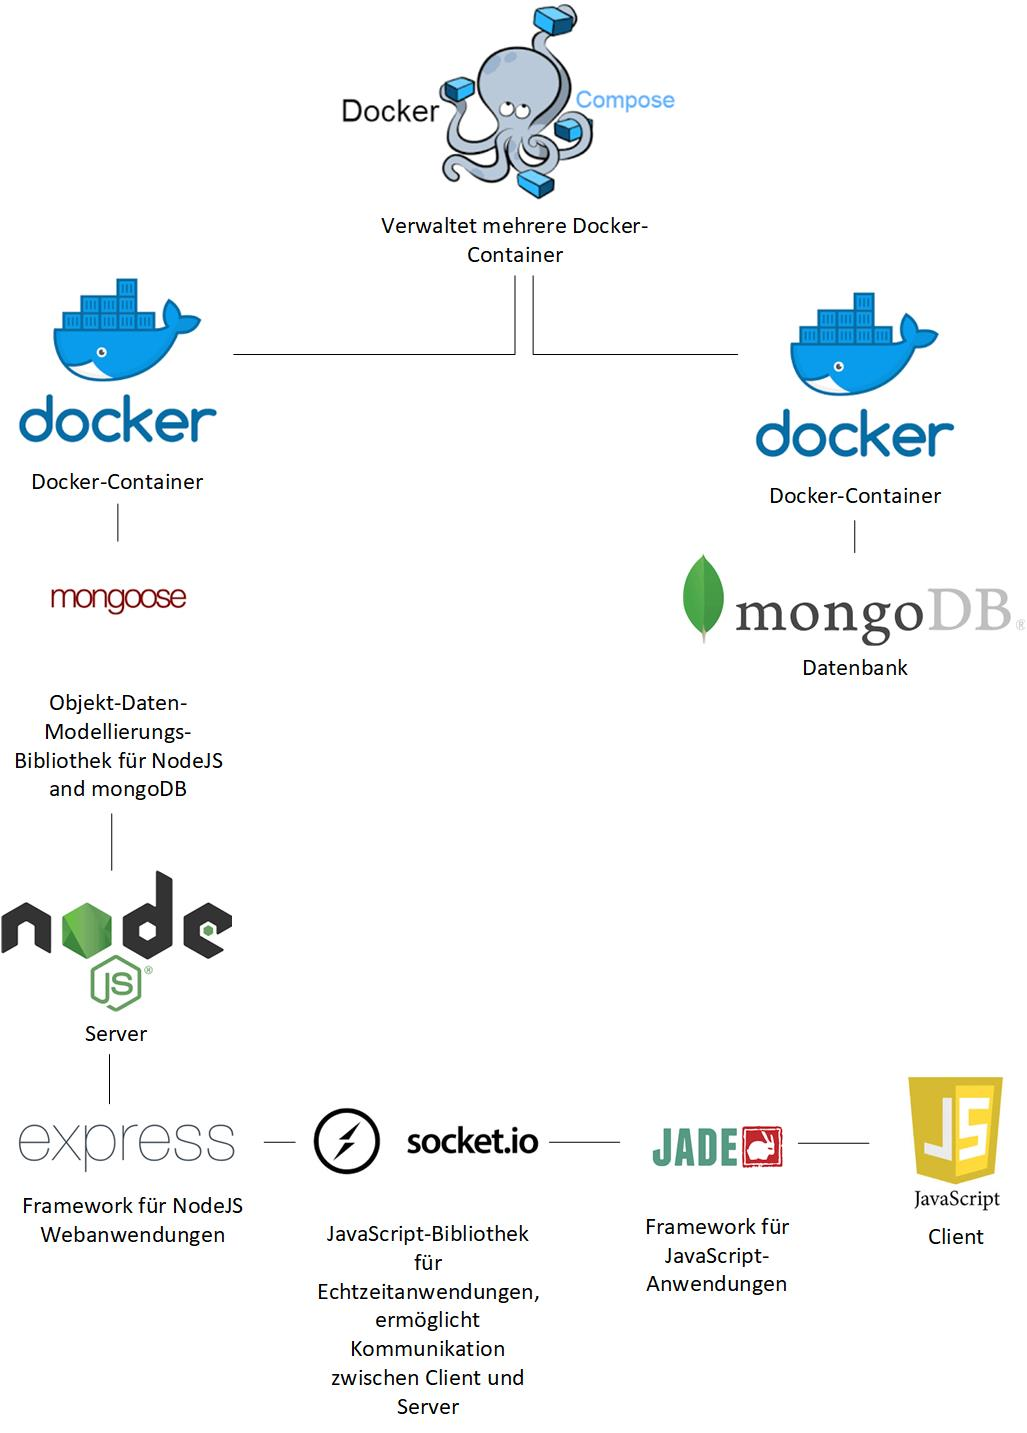
\includegraphics[width=1\textwidth]{images/uebersicht.jpg}
\caption{Übersicht der Anwendung}
\label{fig:koncept}
\end{figure}


\section{Login und Registrierung}\label{sec:Login}
Beim Login hat der User die Möglichkeit, sich zu registrieren oder sich direkt einzuloggen. Die Login-Informationen werden bei der Registrierung in der MongoDB gespeichert und verwaltet. 

\section{Spiel}\label{sec:Spiel}
Nachdem zwei Spieler ein Spiel begonnen haben, können sie gegeneinander spielen. Mittels Buttons kann ausgewählt werden, in welche Reihe sie setzen möchten. Hierbei muss überprüft werden, ob der Spieler an der Reihe ist und ob die Reihe, in der der Stein gesetzt werden soll, nicht voll ist. Außerdem muss geprüft werden, ob es ein Spieler geschafft hat, vier Steine in eine vertikale, horizontale oder diagonale Reihe zu platzieren. Nachdem das Spiel entweder gewonnen oder unentschieden beendet wird, wird das aktuelle Spielfeld deaktiviert und es besteht die Möglichkeit, ein neues Spiel zu starten. Um dem Spieler Informationen über den Spielstand mitzuteilen, schickt ein sogenannter Gamemaster Nachrichten an die Spieler.  Diese Nachrichten werden wie die Chat-Nachrichten über den Websocket geschickt.

Das Spielfeld besteht jeweils aus 7 Spalten und 6 Zeilen, dieses wird als zweidimensionales Array gespeichert. Wenn ein Element den Wert Null hat, bedeutet das, dass kein Spieler an dieser Position einen Stein gesetzt hat.
\section{Nachrichtenfilterung}\label{sec:Nachrichtenfilter}
Typischerweise werden bei einer Websocket-Anwendung allen Usern die eintreffenden Nachrichten angezeigt. Um dies zu umgehen und nur den am Spiel beteiligten Spielern relevante Nachrichten anzuzeigen, enthält die Nachricht die Namen der beiden am Spiel beteiligten Parteien. So kann der Client ermitteln, ob er am Spiel beteiligt ist und aufgrund dessen die Nachrichten anzeigen oder ignorieren. 

\section{Gleichzeitiges Spielen mehrerer Spieler}\label{sec:Multiplegames}
Um es mehr als zwei Spielern zu ermöglichen, gleichzeitig zu spielen, wird ein zweidimensionales Array genutzt. In einer Dimension sind jeweils ein Spielbrett, die zwei Spieler und der Spieler, der aktuell an der Reihe ist, gespeichert. In der anderen Dimension werden die verschiedenen Spiele gespeichert. Sobald ein Spiel beendet wird, werden die zugehörigen Variablen aus dem Array mit dem Wert null belegt. Wenn ein neues Spiel begonnen wird, wird durch das Array iteriert und die erste freie Position verwendet, um dieses Spiel zu speichern. 

	
	% Setup
	%!TEX root = ../dokumentation.tex

%TODO: Einleitung überarbeiten
\chapter{Implementierung}\label{cha:Implementierung}
In diesem Kapitel wird die prototypische Implementierung des Konzepts der Objekterkennung, welches im vorherigen Kapitel beschrieben wurde, behandelt. Diese wird mit Matlab durchgeführt.
\section{Spiellogik}\label{sec:Spiellogik}
	
	% Schlussbetrachtung
	%!TEX root = ../dokumentation.tex

\chapter{Projektabschluss, Fazit \& Ausblick}\label{cha:Schlussbetrachtung}
\section{Fazit}\label{sec:Fazit}
Das Ziel dieser Projektarbeit war die Entwicklung eines Konzepts für eine \ac{LiDAR}-basierte Objekterkennung und eine prototypische Implementierung dieser.
Dazu wurden bereits existierende Clustering-Verfahren diskutiert und deren Vor- und Nachteile für die Verwendung im Kontext dieser Projektarbeit dargestellt. Außerdem wurden konkrete Probleme des \ac{DBSCAN}-Algorithmus mit dem Clustering von \ac{LiDAR}-Daten herausgearbeitet. Diesen wurde durch eine Erweiterung des Algorithmus mit einer distanzabhängigen Berechnung des Parameters $\epsilon$ entgegengewirkt (Kapitel \ref{sec:DBSCAN-Algorithmus_Epsilon}).\\
Die erkannten Objekte werden mit eindeutigen IDs und \ac{AABB}s im Sensordatenbild visualisiert.\\
Zusätzlich wurde eine Tracking-Funktion entwickelt, die das Tracken eines einzelnen Objekts mittels des Kalman-Filter ermöglicht und den Bewegungsverlauf zusätzlich zu den Clustering-Ergebnissen im Sensordatenbild darstellt.
Dieses Konzept wurde mittels Matlab implementiert. Dabei wurde eine Anpassung des \ac{DBSCAN}-Algorithmus vorgenommen, welche die Laufzeit reduziert, da die Analyse eines Messzyklus sonst ca. 70 - 100 Sekunden gedauert hätte (siehe Kapitel \ref{sec:Performance_impl}). Nach der Verbesserung ergaben sich je nach Messumgebung Laufzeiten von ca. 10 - 50 Sekunden.\\
Somit konnten die zu Beginn in Kapitel \ref{sec:Aufgabenstellung} definierten Ziele erreicht werden und zusätzlich die Tracking-Funktion entwickelt werden, die es ermöglicht, nicht nur einen Messzyklus zu analysieren, sondern die zukünftige Position eines Objekts anhand der Analyse vorheriger Messzyklen zu schätzen.
\section{Ausblick}\label{sec:Ausblick}
Es gibt einige Bereiche, in denen die Funktion der Objekterkennung erweitert und verbessert werden kann.\\
Es besteht die Möglichkeit, eine Sensorbewegung in die Berechnungen miteinzubeziehen. Dies bietet sich an, wenn der Sensor auf einem beweglichen Objekt montiert ist. Bisher wurde die Annahme eines stationären Sensors getroffen. Mit einem bewegten Sensor müssten die Koordinaten, die immer relativ zum Sensor aufgenommen werden, in ein Welt-Koordinatensystem umgerechnet werden.
Außerdem könnte die Objekterkennung an Echtzeitanforderungen angepasst werden. Durch die hohe Anzahl an Punkten, die sich in einer Punktwolke befinden, ist die Analyse dieser rechenintensiv. Deshalb müsste voraussichtlich eine Vereinfachung der Sensordaten vor der Analyse vorgenommen werden, um die Ausführungszeit zu reduzieren. Aktuell wird der Matlab-Programmcode für jede Ausführung der Objekterkennung neu interpretiert. Würde der Code der Objekterkennung in ein ausführbares Programm übersetzt werden, so ließe sich die Ausführungszeit weiter reduzieren.\\
In Bezug auf die Tracking-Funktionalität ist es denkbar, diese um ein Tracking von mehreren Objekten zu erweitern. Dazu müsste eine neue Strategie zur Data-Association entwickelt werden. Es ist dabei zu beachten, dass die Tracking-Funktion auf das Tracken von Personen ausgerichtet ist. Sollen auch Objekte anderer Art getrackt werden, so muss auch ggf. eine Anpassung des Bewegungsmodells für den Kalman-Filter in Betracht gezogen werden.\\
Neben der Funktion des Trackens mehrerer Objekte könnte das Tracking um die Funktion eines automatischen Starts des Trackings erweitert werden. Bisher wählt der Benutzer aus, welches Objekt getrackt werden soll. Durch eine Analyse, welche Objekte beweglich sind, könnte dieser Prozess automatisiert werden, sodass keine Benutzereingabe mehr erforderlich ist.
 
	
	% Fazit
%	\input{content/Fazit.tex}

	% Inhalt
	%\foreach \i in {01,02,03,04,05,06,07,08,09,...,99} {%
	%	\edef\FileName{content/\i kapitel}%
	%		\IfFileExists{\FileName}{%
	%			\input{\FileName}
	%		}
	%		{%
	%			%file does not exist
	%		}
	%}

	\clearpage
		
	\pagenumbering{roman}
	
	% Literaturverzeichnis
	\cleardoublepage
	\printbibheading
	\printbibliography[nottype=online,heading=subbibliography,title={Publikationen}]
	\printbibliography[type=online,notkeyword=Gesetz,notkeyword=Standard,heading=subbibliography,title={Online Quellen}]	\printbibliography[type=online,keyword=Gesetz,heading=subbibliography,title={Rechtsquellenverzeichnis}]
\printbibliography[type=online,keyword=Standard,heading=subbibliography,title={Standards \& Normen}]
	
%	\renewcommand\bibname{Literaturverzeichnis}
%	\printbibliography

%	\newpage\null\thispagestyle{plain}\newpage
	

	
	% sonstiger Anhang
	\clearpage
	\appendix
	% !TeX root = ../dokumentation.tex

\addchap{\langanhang}


\section*{A. Nachweis der Funktionalität}\label{sec:NachweisFunktionalitaet}

\pagebreak

 
	
\end{document}
